% WURC Hardware Introduction
\section{Introduction}
\label{sec_hw_intro}

	When \ac{TVWS} radio spectrum was first released for unlicensed use, the only systems that were available for operation on this band were early prototypes from Microsoft \cite{yuan2007knows} and Adaptrum \cite{ko2014television}, as well as a few other frequency-shifted single-radio, single-carrier modulation systems from several vendors \cite{ko2014television}. 

	In fact, we evaluate the performance of our own prototype legacy \ac{SISO} \ac{TVWS} system in Section~\ref{sec_siso_tvws} and show that while propagation of 802.11-like \ac{TVWS} systems is much improved compared to similar 802.11 networks operating in 2.4 and 5.8~GHz \ac{ISM} bands, system performance is significantly decreased due to the limited practical channel bandwidth available in \ac{TVWS}.\footnote{It was only in 2015 that final rules were issued by the FCC that enabled \ac{TVWS} systems to bond multiple 6~MHz TV channels within the United States \cite{fcc2015ro}.}
		
	At the time, no radio platform existed that: 1) allowed us to transmit at 1~Watt or greater within \ac{TVWS} bands; 2) allowed access to the \ac{PHY} layer for \ac{CSI}, precoding, and modification of the \ac{PHY} itself; and most importantly, 3) could be configured for large-scale, real-time, and \emph{mobile} \ac{MU-MIMO} operation.
	
	% WURC Prototypes
\begin{figure}[ht]
\centering
  	\includegraphics[width=1\linewidth]{figs/wurc/wurc_versions}   
   	\caption{Three revisions of the Wideband UHF Radio Card (WURC) prototype.
	\label{fig_wurc_versions}}
\end{figure}

	Therefore, in this chapter, we seek to design, implement, and test a new radio system that meets the above criteria for providing broadband connectivity over \ac{TVWS} channels.
	
	To this end, we present the \acf{WURC}, the first software-defined radio platform that implements 802.11af-like operation and \ac{MU-MIMO} beamforming \cite{WURC} (Figure~\ref{fig_wurc_versions}).
	When implemented in a larger system, \ac{WURC} is able to leverage an unprecedented tuning range for \ac{MU-MIMO} systems between 50 - 5875~MHz, enabling direct comparison of key \ac{MU-MIMO} performance metrics across \emph{two octaves} of radio spectrum.
	
	In order to realize this new experimental platform, we had to solve several key physical layer design challenges to enable agile, wideband operation, fast transit/receive switching required for the 802.11 \ac{DCF} protocol, and distributed clock and timing synchronization issues that limited the scalability of our system in particular and \ac{MU-MIMO} systems in general.
	
	These solutions are implemented on a new, modular PCB-based \ac{SDR} platform shown in Figure~\ref{fig_wurc_versions} that we designed, manufactured, and tested. Over 50 \ac{WURC} systems were manufactured and used in over a dozen research labs around the world for \ac{TVWS} system prototyping.
		
	This hardware platform was operated with an extensive and modular software command and control library that leverages the open-source WARP project to implement its \ac{PHY} rapid-prototyping experimental framework and real-time 802.11af-like communications framework \cite{warpProject}.

	%We first present a high-layer overview of \acp{WURC} modular architecture and construction, discuss the various \ac{PHY} design challenges and solutions we develop for \ac{WURC}.
	After describing the basic \ac{WURC} radio module, we will present several \ac{MU-MIMO} experimental platforms built with \ac{WURC} that enable us to achieve our large-scale \ac{TVWS} system design goals.


%##############################################################################
\section{WURC High-Level System Design}
\label{sec_wurc_module}

	\ac{MU-MIMO} systems generally require a large number of transmit and receive RF chains on the \ac{AP} to generate multiple spatial streams; these radios must be coherent (\emph{i.e.} share the same RF reference clock).
	In addition, a large number of distributed \ac{STA} nodes are required to serve as the clients to the \ac{AP}.
	Given that we wished to implement the complete 8x8 \ac{MU-MIMO} 802.11af standard with accessibility and programmability across the entire network stack, we decided to implement our own \ac{SDR} platform, \ac{WURC} that could be produced in large numbers.

% WURC hardware key features
\begin{figure}[ht]
\centering
  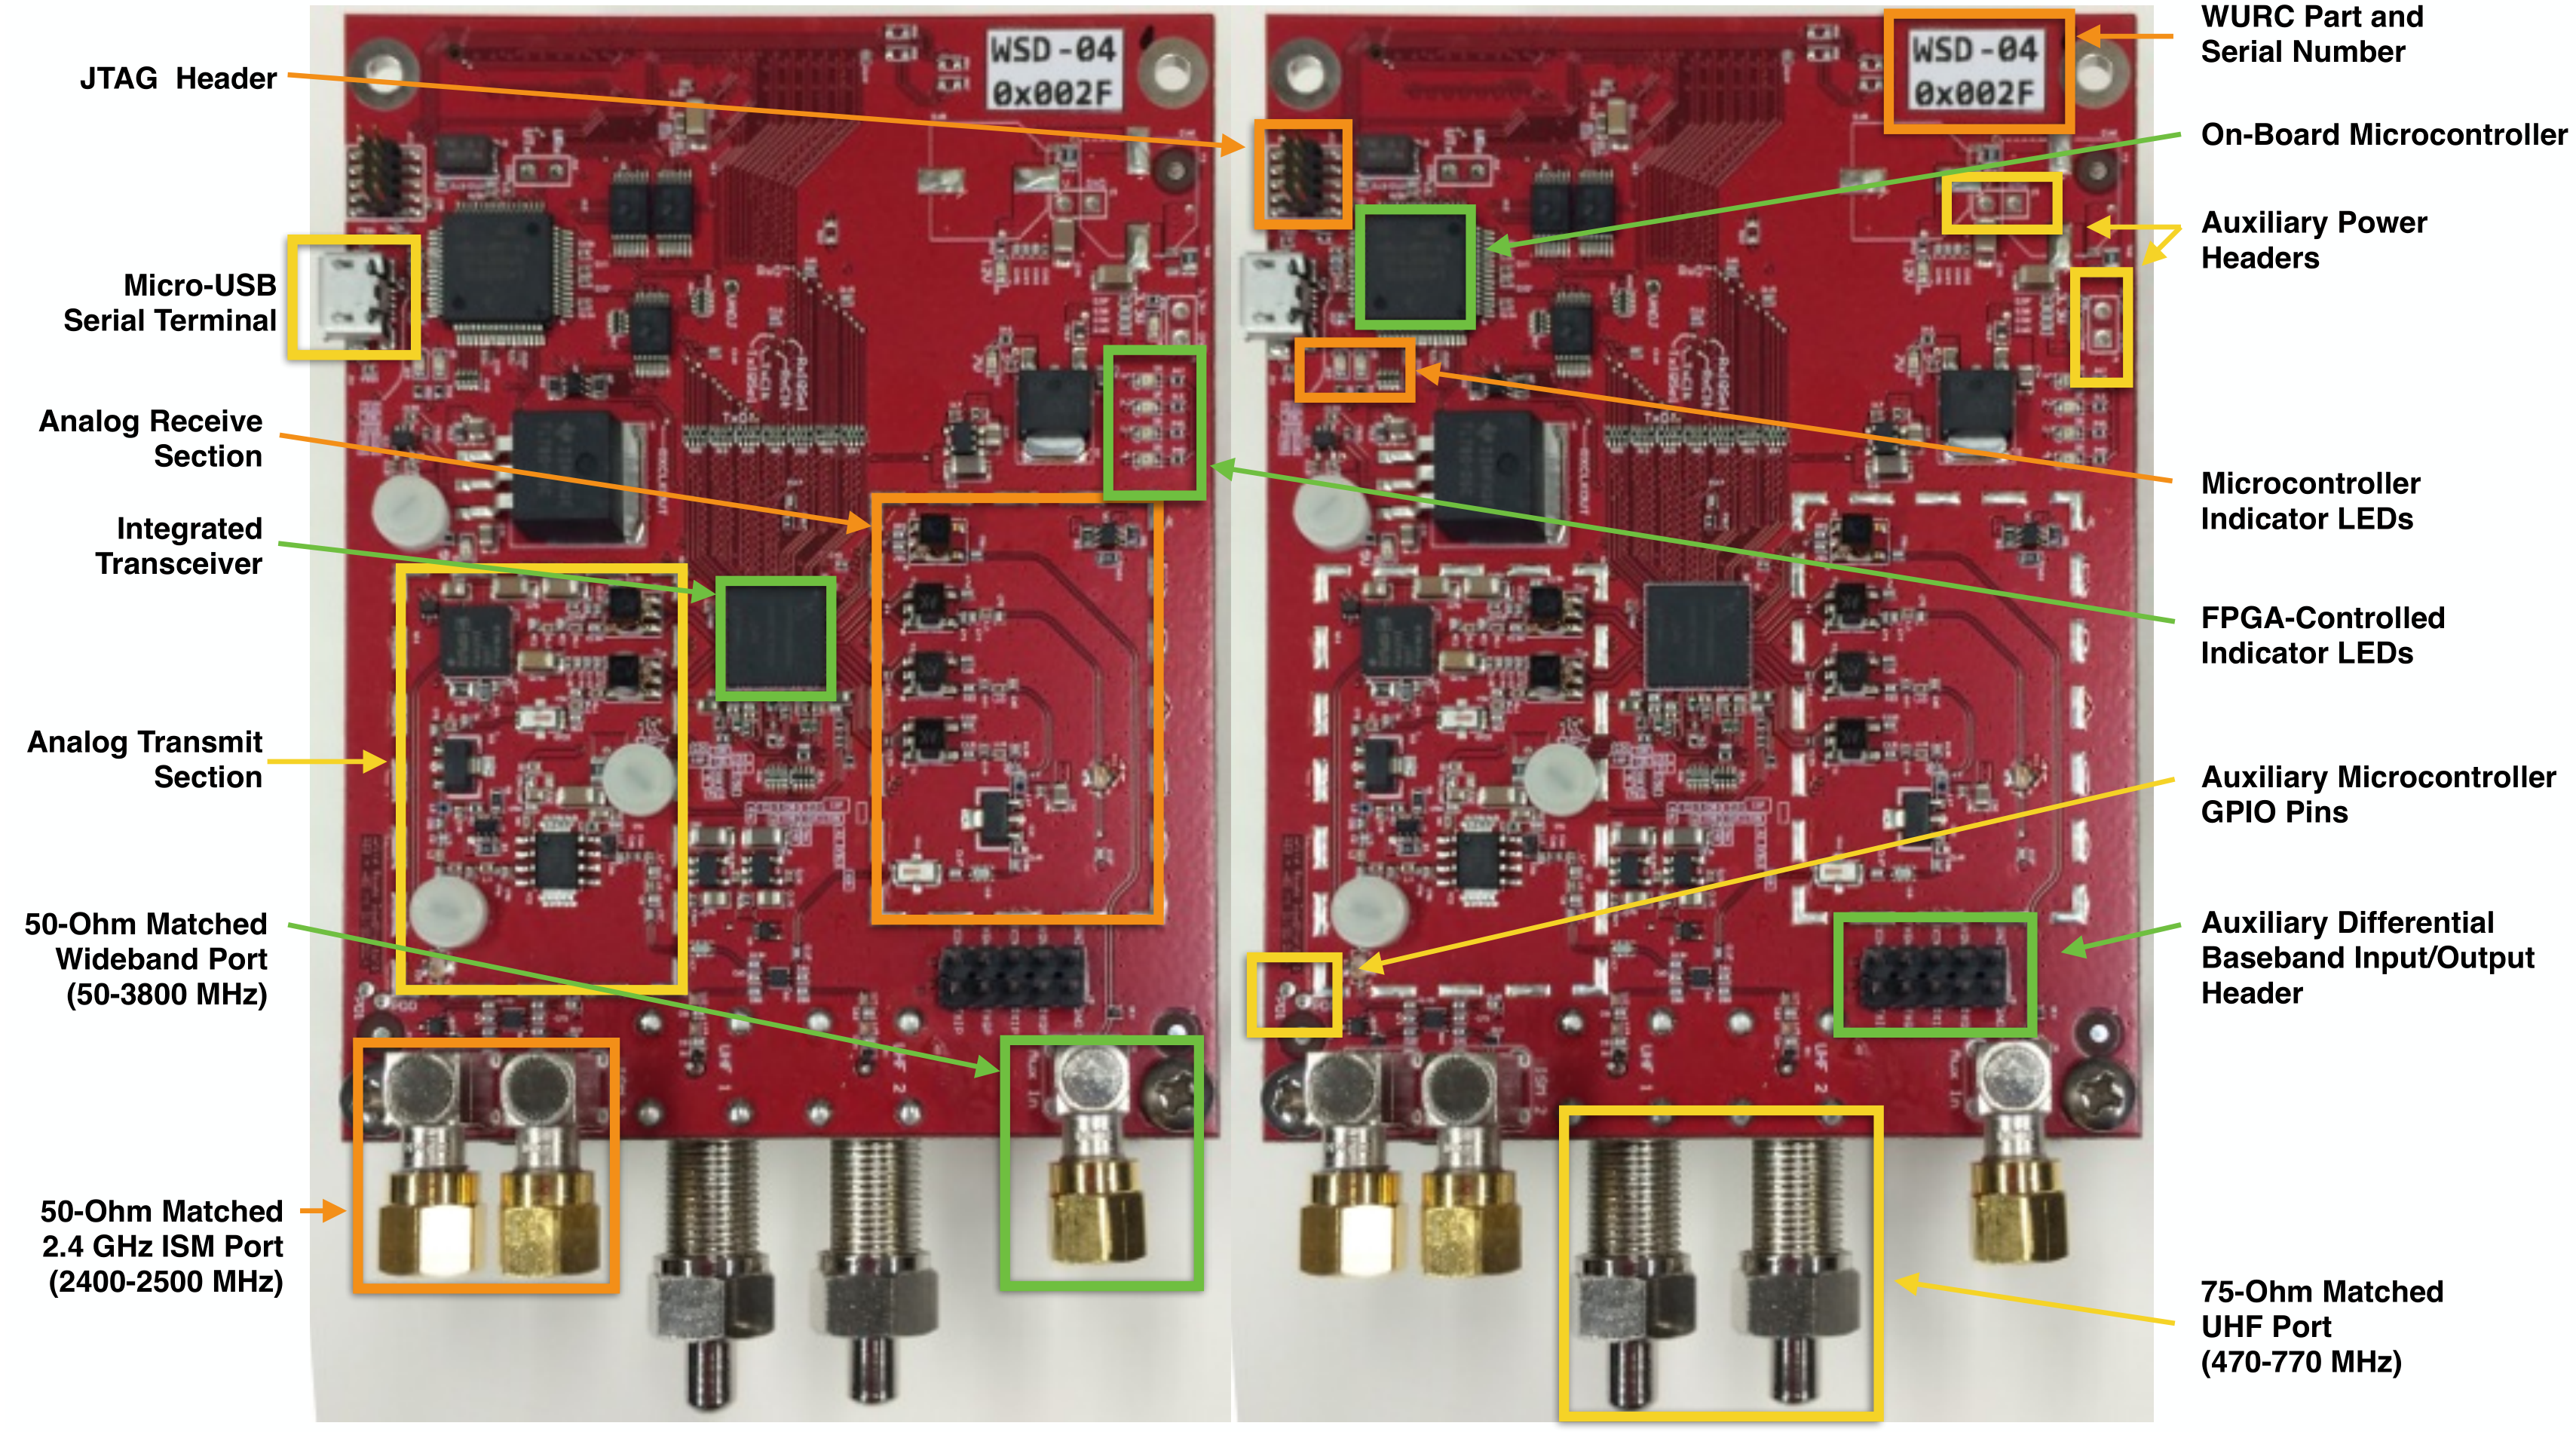
\includegraphics[width=1\linewidth]{figs/wurc/wurc_detailed_components}   
    \caption{A Wideband UHF Radio Card (WURC) with sections labeled.}
\label{fig_wurc_hw_diagram}
\end{figure}

	\ac{WURC} is a software-defined radio daughter-card, designed to present an abstracted 12-bit quadrature I/Q parallel interface and a serial control console to the host system.
	By designing each \ac{WURC} board as a self-calibrating, self-configuring radio head, we simplified the system architecture and made each unit modular.
	The layout and various important features of the \ac{WURC} \ac{SDR} module can be seen in Figure~\ref{fig_wurc_hw_diagram}, where notably a 50~$\Omega$ port for 2.4~GHz \ac{ISM}-band operation and a 75~$\Omega$ port for UHF-band operation are the primary antenna interfaces.
	
	We designed \ac{WURC} to implement the \textit{direct-conversion} \acf{FPRF} LMS6002D system from Lime Microsystems \cite{lime2012lms6002d}, which integrates frequency synthesis, quadrature digital/analog conversion, baseband filters, RF mixing, and programmable gain controls into a single integrated circuit.
		This minimizes size, implementation complexity, and energy-consumption of the radio transceiver chain while providing significant flexibility regarding analog RF properties.
	The LMS6002D is configured through a 4-wire serial interface into an 8-bit register space.
	In order to simplify the management of a large number of radio chains,  \ac{WURC} is designed to be modular, with calibration/control libraries and board-dependent calibration tables stored locally on each daughter-card on a Texas Instruments LM3S5R36 microcontroller \cite{ti2012stellaris} and controlled through a simplified \ac{UART} interface.
	This eases the requirements for integration with a host platform and makes the radio daughter-cards completely interchangeable.
	A simplified block diagram showing input and output data paths is shown in Figure~\ref{fig_wurc_block_diagram}.
	
	Some of the important system parameters that will be used in this thesis are available in Table~\ref{tab_wurc_specs}; additional hardware details can be found in the relevant hardware specification sheets \cite{lime2012lms6002d, ti2012stellaris}.

% Table generated by Excel2LaTeX from sheet 'Sheet1'
\begin{table}[htbp]
  \centering
  \caption{Important system parameters for \acf{WURC}}
%\resizebox{0.6\textwidth}{!}{%
    \begin{tabular}{|lrl|}
    \toprule
    \rowcolor[rgb]{ .31,  .506,  .741} \multicolumn{1}{|c}{\textcolor[rgb]{ 1,  1,  1}{\textbf{Parameter}}} & \multicolumn{1}{c}{\textcolor[rgb]{ 1,  1,  1}{\textbf{Value}}} & \multicolumn{1}{c|}{\textcolor[rgb]{ 1,  1,  1}{\textbf{Unit}}} \\
    \midrule
    \rowcolor[rgb]{ .863,  .902,  .945} \multicolumn{1}{|c}{\textbf{RF Transceiver}} & \multicolumn{1}{c}{\textbf{LMS6002D} \cite{lime2012lms6002d}} &  \\
    \midrule
    Tuning Range & 50 - 3800 & MHz \\
    \midrule
    \rowcolor[rgb]{ .863,  .902,  .945} Output Power (UHF) & 30    & dBm CW \\
    \midrule
    Output Power (ISM) & 27    & dBm CW \\
    \midrule
    \rowcolor[rgb]{ .863,  .902,  .945} ADC Bits & 12    & bits \\
    \midrule
    ADC Sampling Rate & 40    & MSps \\
    \midrule
    \rowcolor[rgb]{ .863,  .902,  .945} SFDR  & 60    & dBc \\
    \midrule
    DAC Bits & 12    & bits \\
    \midrule
    \rowcolor[rgb]{ .863,  .902,  .945} DAC Sampling Rate & 40    & MSps \\
    \midrule
    SPI Bus Rate & 50    & MHz \\
    \midrule
    \rowcolor[rgb]{ .863,  .902,  .945} \multicolumn{1}{|c}{\textbf{Microcontroller}} & \multicolumn{1}{c}{\textbf{TI LM3S5R36} \cite{ti2012stellaris}} &  \\
    \midrule
    Processor & ARM Cortex-M3 & - \\
    \midrule
    \rowcolor[rgb]{ .863,  .902,  .945} Clock Speed & 80    & MHz \\
    \midrule
    Debug Interface & Micro-USB, JTAG & - \\
    \midrule
    \rowcolor[rgb]{ .863,  .902,  .945} SPI Write Speed & 40    & MHz \\
    \midrule
    SPI Read Speed & 10    & MHz \\
    \bottomrule
    \end{tabular}%
%}
  \label{tab_wurc_specs}%
\end{table}%


% WURC block diagram
\begin{figure}[p]
\centering
  \includegraphics[width=0.7\linewidth]{figs/wurc/WARP_WURC}   
    \caption{Block diagram of WURC module on a host WARPv3 board.}
\label{fig_wurc_block_diagram}
\end{figure}

% WURC block diagram
\begin{figure}[p]
\centering
  \includegraphics[width=0.7\linewidth]{figs/wurc/wurc_platform_rev_a_warp}   
    \caption{WARPv3 SDR platform, HSMC/FMC adaptor, and WURC SDR platform.}
\label{fig_warp_wurc_hw}
\end{figure}

	\ac{WURC} physically connects to a host via an HSMC or FMC (with custom adapter board) daughter-card slot, and provides a 12-bit digital baseband quadrature interface to the host system (Figure~\ref{fig_wurc_block_diagram}).
	This permits in-field reconfiguration of RF analog parameters such as channel bandwidth and center frequency between 300-3800 MHz, though the analog transmit and receive paths are currently optimized and calibrated for transmissions between 470-798 MHz on the UHF antenna ports, and 2400-2500 MHz on the ISM antenna ports.

	The daughter-card is powered by the 12V HSMC standard voltage rail, with all additional voltages and power filtering circuits contained on the daughter-card.

	We designed and tested fast-switching control circuits on the discrete amplification stages that allow the system to operate as a \ac{TDD} transceiver with a switching time of less than 7~$\mu$s, or an \ac{FDD} transceiver with independent transmit and receive fractional-N frequency synthesizers.
	Since our primary interest was to operate the \ac{WURC} as a \ac{TDD} 802.11af radio, we designed in two RF ports, one transmit/receive and one dedicated receive, which would allow the addition of an external duplexer for \ac{FDD} operation to a single antenna, if desired.
	For the rest of this thesis, we will focus on \ac{TDD} applications.
	
\subsubsection{WARP Framework Integrations}
\label{sec_warp_mods}

	WARPv3 is an open-source hardware platform for prototyping \ac{SDR} systems with a large Xilinx Virtex-6 LX240T FGPA, transceivers for 2.4 and 5.8~GHz ISM-bands, software reference designs, MATLAB integration \cite{warpProject}, and most importantly, a VITA 57.1 FMC expansion connector \cite{samtec2018vita}.
	With an intermediate adaptor \ac{PCB} that we designed and manufactured to translate between the HSMC and FMC mezzanine connector standards, we are able to interface our \ac{WURC} daughter-card to a host WARPv3 system shown in Figure~\ref{fig_warp_wurc_hw}.
	In the WARPv3 \ac{FPGA}, we multiplex radio control signals and digital quadrature I/Q streams between the built-in ISM-band radios and WURC's UHF transceivers.

	A standards-compliant 802.11 \acf{MAC} and \acf{PHY} implementation has been developed for the WARPv3 platform \cite{warp80211}, which we use as a starting point for our real-time 802.11af implementation \cite{flores2013ieee80211af}.
	From the perspective of the WARP 802.11 digital baseband, the analog front-end is transparent, which allows an interchangeable \emph{analog} \ac{PHY} to be used with the same digital MAC/PHY for fair comparison.
	This is especially useful for MU-MIMO comparison studies across ISM bands as this re-used of the digital MAC/PHY controls for a large number of variables in the radio chain.

\subsubsection{Adjustable Channel Bandwidth}
\label{sec_warp_chan_bw}

	The 802.11 reference design operates by default in a 20~MHz channel bandwidth.
	In order to enable a UHF transmission to fit within one or two contiguous UHF channels of 6~MHz, we modify the 802.11 reference design to operate at 10 and 5~MHz channel bandwidths in compliance with the 802.11af standard \cite{warp80211}.
	This is accomplished by reducing the data sampling rate by $\frac{1}{2}$ and $\frac{1}{4}$, respectively, with new programmable decimation filters added to the WARPv3 reference \ac{FPGA} design and adjusting \ac{MAC} timing parameters and receiver \ac{DSP} blocks to match.
	
		Now that we've presented the high-level overview of the designed \ac{WURC} \ac{TVWS} radio module, we will now dive in to some of the important \ac{PHY} problems and solution that were required to realize this platform before rounding out this chapter with a discussion of software architecture design for scaling from 1x1 up to 8x8 and larger \ac{MU-MIMO} arrays.

